\chapter{Arhitektura i dizajn sustava}
			
			
			Odabir odgovarajuće arhitekture je važna odluka koja utječe na cjelokupnu funkcionalnost sustava. Budući da je cilj aplikacije široka dostupnost, odabrali smo web aplikaciju. Web aplikacija funkcionira neovisno o platformi, što oslobađa razvojni tim višeplatformnog razvoja.\\
			Korisnik aplikaciji pristupa pomoću web preglednika. Web preglednik je program koji omogućava korisniku pregled i prikaz web aplikacije na uređaju. Kako bi se omogućila komunikacija klijenta(korisnika) s aplikacijom koristi se web poslužitelj koji koristi HTTP protokol. Aplikacija komunicira sa backend-om preko REST API-ja. Backend dohvaća sve potrebne podatke iz baze podataka(više o njoj u sljedećoj sekciji) nakon čega preko poslužitelja i preglednika prikazuje te podatke korisniku u obliku HTML dokumenta.\\
			Aplikacija je pisana u programskom jeziku Java i programskom okruženju Spring Boot, te React-u(JavaScript biblioteka za izgradnju korisničkih sučelja), a od razvojnih okruženja odabrali smo Visual Studio Code za frontend  te IntelliJ IDEA za ostatak posla.\\
			
Logika backenda izgrađena je na temelju REST konvencije, stoga je razrađena u tri sloja: Repository, Service i Controller. 
			\begin{itemize}
				\item \textbf{Repository} – Sloj Repository primarno je zadužen za komunikaciju s bazom podataka. U njemu se nalaze standardne metode za dohvaćanje, spremanje i izmjenu podataka u bazi. Te metode temelje se na atributima entiteta za koji je izgrađen pojedini repository. Također, svaki repository može biti nadopunjen vlastitim metodama.
				\item \textbf{Service} – U Service sloju odvija se poslovna logika i manipulacija podacima koji dolaze s baze. To uključuje kreiranje klasa, promjenu tipova, omatanje i sl. 
				\item \textbf{Controller} –  prima i obrađuje zahtjeve poslužitelja. Svi se zahtjevi prosljeđuju koristeći JSON format. Shodno pojedinom zahtjevu, controller zatražuje podatke sa repositoryja, izvodi metode koje mu pruža Service. Na kraju podatke u obliku objekata šalje kao odgovor web poslužitelju.  
			\end{itemize}
			React je javascript knjižnica za izgradnju korisničkih sučelja. Temelji se na deklariranju komponenata koje se prikazuju korisniku preko web preglednika.
			\begin{figure}
				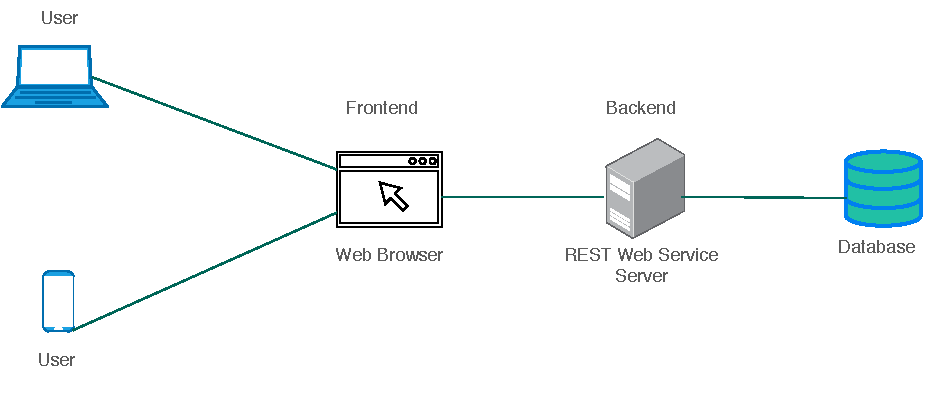
\includegraphics{Arhitektura_sustava}
				\caption{Arhitektura sustava}
			\end{figure}
			
			
			
			\section{Baza podataka}

			Sve je podatke potrebno negdje spremiti kako bi se mogli dinamički dohvaćati. Za ovo nam služi baza podataka, koju također smatramo dijelom MVC obrasca. Naša aplikacija u pozadini koristi, kao relacijsku bazu podataka, PostgreSQL.
			\\
			U bazi podataka nalaze se sljedeći entiteti:
			\begin{itemize}
				\item Korisnik
				\item Adresa
				\item Ocjena
				\item Zahtjev
				\item Obavijest
				\item Potencijalni
			\end{itemize}
			
			\subsection{Opis tablica}
			
			
			\textbf{Korisnik} Ovaj entitet modelira jednog korisnika aplikacije.\\
			Sadrži atribute: korisnikID, ime, prezime, e-posta, lozinka, korisnickoIme, jeAdmin, telefon, slika, status, i
			adresaID koji predstavlja strani ključ na entitet Adresa. Korisnik je povezan s entitetom Ocjena vezama "prima" i "daje" (\textit{One-to-Many}) preko atributa korisnikID. Korisnik se također veže s entitetom Zahtjev vezama "autorski" i "izvršiteljski" (\textit{One-to-Many}) preko atributa korisnikID i vezom "potencijalni" (\textit{Many-to-Many}) preko atributa korisnikID. Ovaj entitet se još veže uz entitet Adresa vezom \textit{Many-to-One} preko atributa adresaID. Također je u vezi s entitetom Obavijest vezom \textit{One-To-Many} preko atributa korisnikID.
			
			\begin{tabularx} {\textwidth} {|p{3.5cm}|p{2cm}|X|}
				
				\hline
				\multicolumn{3}{|c|}{\textbf{Korisnik}} \\
				\hline
				
				
				\cellcolor{LightGreen}korisnikID & INT	&   jedinstveni identifikator svakog korisnika 	\\ \hline
				ime	& VARCHAR &   ime korisnika	\\ \hline 
				prezime & VARCHAR &  prezime korisnika \\ \hline 
				e-posta & VARCHAR	&  	e-mail adresa korisnika	\\ \hline 
				lozinka & VARCHAR	&  	hash lozinke	\\ \hline
				korisnickoIme & VARCHAR	&  	korisnicko ime	\\ \hline
				jeAdmin & BOOLEAN	&  	oznaka je li korisnik administrator	\\ \hline
				telefon & VARCHAR	&  	broj mobitela korisnika	\\ \hline
				slika & BOOLEAN	&  	oznaka je li korisnik ima sliku profila	\\ \hline
				status & VARCHAR	&  	oznaka statusa korisničkog računa	\\ \hline
				\cellcolor{LightBlue}adresaId & VARCHAR	&  	adresa prebivališta korisnika	\\ \hline
				
				
				
			\end{tabularx} 
			
			\bigskip
			\bigskip
			\textbf{Adresa} Ovaj entitet modelira adresu prebivališta pojedinog korisnika aplikacije.
			Sadrži sljedeće atribute: adresaID, opis, xKoordinata, yKoordinata. Entitet Adresa je u vezi \textit{One-to-Many} s entitetom Zahtjev preko atributa adresaID i u vezi \textit{One-to-Many} s entitetom Korisnik pomoću atributa adresaID.
			\bigskip
			
			
			\begin{tabularx} {\textwidth} {|p{3.5cm}|p{2cm}|X|}
				
				\hline
				\multicolumn{3}{|c|}{\textbf{Adresa}} \\
				\hline
				
				\cellcolor{LightGreen}adresaID & INT	& jedinstveni identifikator adrese korisnika	\\ \hline 
				opis & VARCHAR & Detaljniji opis adrese korisnika  \\ \hline 
				xKoordinata & NUMERIC	& X koordinata adrese korisnika predočena na karti	\\ \hline 
				yKoordinata & NUMERIC	& Y koordinata adrese korisnika predočene na karti		\\ \hline
				
				
				
			\end{tabularx}
			
			\bigskip
			\bigskip
			\textbf{Ocjena} Ovaj entitet predstavlja ocjenu koju jedan korisnik daje drugome. Sadrži atribute: ocjenaID, komentar, ocjena, korisnikID, zahtjevID, primakorisnikID. Ovaj entite sadrži tri strana ključa, a to su: korisnikID(predstavlja korisnika koji ocjenjuje), primakorisnikID(predstavlja korisnika kojeg se ocjenjuje) i zahtjevID(predstavlja zahtjev koji se izvršava). Ocjena je u  dvije veze s entitetom Korisnik, a to su "prima" (\textit{Many-to-One}) i "daje" (\textit{Many-to-One}) preko atributa korisnikID. Ocjena se još veže uz Zahtjev vezom \textit{One-to-One} preko atributa zahtjevID. 
			\bigskip
			
			\begin{tabularx} {\textwidth} {|p{3.5cm}|p{2cm}|X|}
				
				\hline
				\multicolumn{3}{|c|}{\textbf{Ocjena}} \\
				\hline
				
				\cellcolor{LightGreen}ocjenaID & INT	& jedinstveni identifikator svake ocjene	\\ \hline
				komentar	& VARCHAR &  komentar kojeg korisnik ostavlja uz ocjenu 	\\ \hline 
				ocjena & INT & ocjena koju korisnik dodjeljuje  \\ \hline 
				\cellcolor{LightBlue} korisnikID	& INT &  korisnik koji ocjenjuje 	\\ \hline 
				\cellcolor{LightBlue} zahtjevID	& INT &  zahtjev koji se izvršava 	\\ \hline 
				\cellcolor{LightBlue} primakorisnikID	& INT &  korisnik kojeg se ocjenjuje 	\\ \hline 
				
			\end{tabularx}
			
			\bigskip
			\bigskip
			\textbf{Zahtjev} Ovaj entitet predstavlja jedan zahtjev kojeg korisnik aplikacije zadaje ili izvršava. Sadrži atribute:zahtjevID, opis, datumVrPocetka, naslov, datumIsteka, status, adresaID, korisnikID, autorskikorisnikID. Kao i entitet ocjena i ovaj entitet sadrži tri strana ključa: adresaID(predstavlja adresu korisnika koji je zadao zahtjev, nije obavezno kako bi se kreirao zahtjev), korisnikID(predstavlja izvršitelja zahtjeva) i autorskikorisnikID(predstavlja samog kreatora zahtjeva). Entitet je u vezi s Ocjenom preko veze \textit{One-to-One} pomoću atributa zahtjevID. Zahtjev se veže uz entitet Korisnik preko tri veze "autorski" (\textit{Many-to-One}), veze "izvršiteljski" (\textit{Many-to-One}) i veze "potencijalni" (\textit{Many-to-Many}) svaka preko atributa korisnikID. Još se veže uz entitet Adresa \textit{One-to-Many} preko atributa adresaID. Također je u vezi s entitetom Obavijest vezom \textit{One-To-Many} preko atributa zahtjveID. 
			\bigskip
			
			\begin{tabularx} {\textwidth} {|p{3.5cm}|p{2cm}|X|}
				
				\hline
				\multicolumn{3}{|c|}{\textbf{Zahtjev}} \\
				\hline
				
				\cellcolor{LightGreen}zahtjevID & INT	& jedinstveni identifikator svakog zahtjeva	\\ \hline
				opis	& VARCHAR &  opis zahtjeva 	\\ \hline 
				datumVrPocetka & DATETIME &  trenutak postavljanja zahtjeva na aplikaciju \\ \hline 
				datumIsteka & DATE	&  datum kada zahtjev istječe, te se ne može više izvršavati		\\ \hline
				naslov & VARCHAR	&  naslov zahtjeva
				\\
				\hline
				status & VARCHAR & status zahtjeva  \\ \hline
				\cellcolor{LightBlue} adresaID	& INT &  adresa autora zahtjeva 	\\ \hline 
				\cellcolor{LightBlue} korisnikID	& INT &  izvršitelj zahtjeva 	\\ \hline
				\cellcolor{LightBlue} autorskikorisnikID	& INT &   autor zahtjeva	\\ \hline
				
				
			\end{tabularx}
			
			\bigskip
			\bigskip
			\textbf{Potencijalni} Ovaj entitet predstavlja sve potencijalne izvršitelje jednog zahtjeva. Sadrži atribute: zahtjevID, korisnikID. Oba atributa su strani ključevi. Prvi predstavlja zahtjev kojeg korisnik želi izvršiti, drugi predstavlja korisnika koji želi izvršit zahtjev. Ovaj entitet nastaje radi \textit{Many-to-Many} veze "potencijalni" između Zahtjeva i Korisnika.
			\bigskip
			
			\begin{tabularx}{\textwidth} {|p{2cm}|p{2cm}|X|}
				\hline
				\multicolumn{3}{|c|}{\textbf{Potencijalni}} \\
				\hline
				\cellcolor{LightGreen} zahtjevID & INT & zahtjev kojeg korisnik želi izvršiti \\
				\hline
				\cellcolor{LightGreen} korisnikID & INT & potencijalni izvršitelj zahtjeva \\
				\hline
			\end{tabularx}
			
			\bigskip
			\bigskip
			\textbf{Obavijest} Ovaj entitet predstavlja sve moguće obavijesti koje jedan korisnik može dobiti. Sadrži atribute: obavijestID, korisnikID,
			poruka, zahtjevID, jeliPročitana. Ovaj entite sadrži dva strana ključa: korisnikID(predstavlja korisnika kojem je obavijest namijenjena), te zahtjevID(predstvavlja zahtjev na kojeg se obavijest odnosi). Entitet je u vezi s entitetom Korisnik vezom \textit{Many-To-One} pomoću atributa korisnikID, te s entitetom Zahtjev vezom \textit{Many-To-One} preko atributa zahtjevID.
			\bigskip
			
			\begin{tabularx}{\textwidth} {|p{2.4cm}|p{2cm}|X|}
				\hline
				\multicolumn{3}{|c|}{\textbf{Obavijest}} \\
				\hline
				\cellcolor{LightGreen} obavijestID & INT & jedinstveni identifikator obavijesti \\
				\hline
				poruka & VARCHAR & predstavlja detaljniji opis obavijesti \\
				\hline
				jeliPročitana & BOOLEAN & označuje jeli korisnik pročitao obavijest \\
				\hline
				\cellcolor{LightBlue}
				korisnikID & INT & korisnik kojem je obavijest namijenjena. \\
				\hline
				\cellcolor{LightBlue}
				zahtjevID & INT & zahtjev na kojeg se obavijest odnosi \\
				\hline
			\end{tabularx}
			
			
			
			\newpage
			\subsection{Dijagram baze podataka}
			Podcrtani elementi su ključevi, elementi koji imaju (O) nisu obavezni za unos u bazu podataka, elementi koji imaju (FK) su strani ključevi i elementi s oznakom (U) moraju biti jedinstveni.
			
			\begin{figure}[h]
				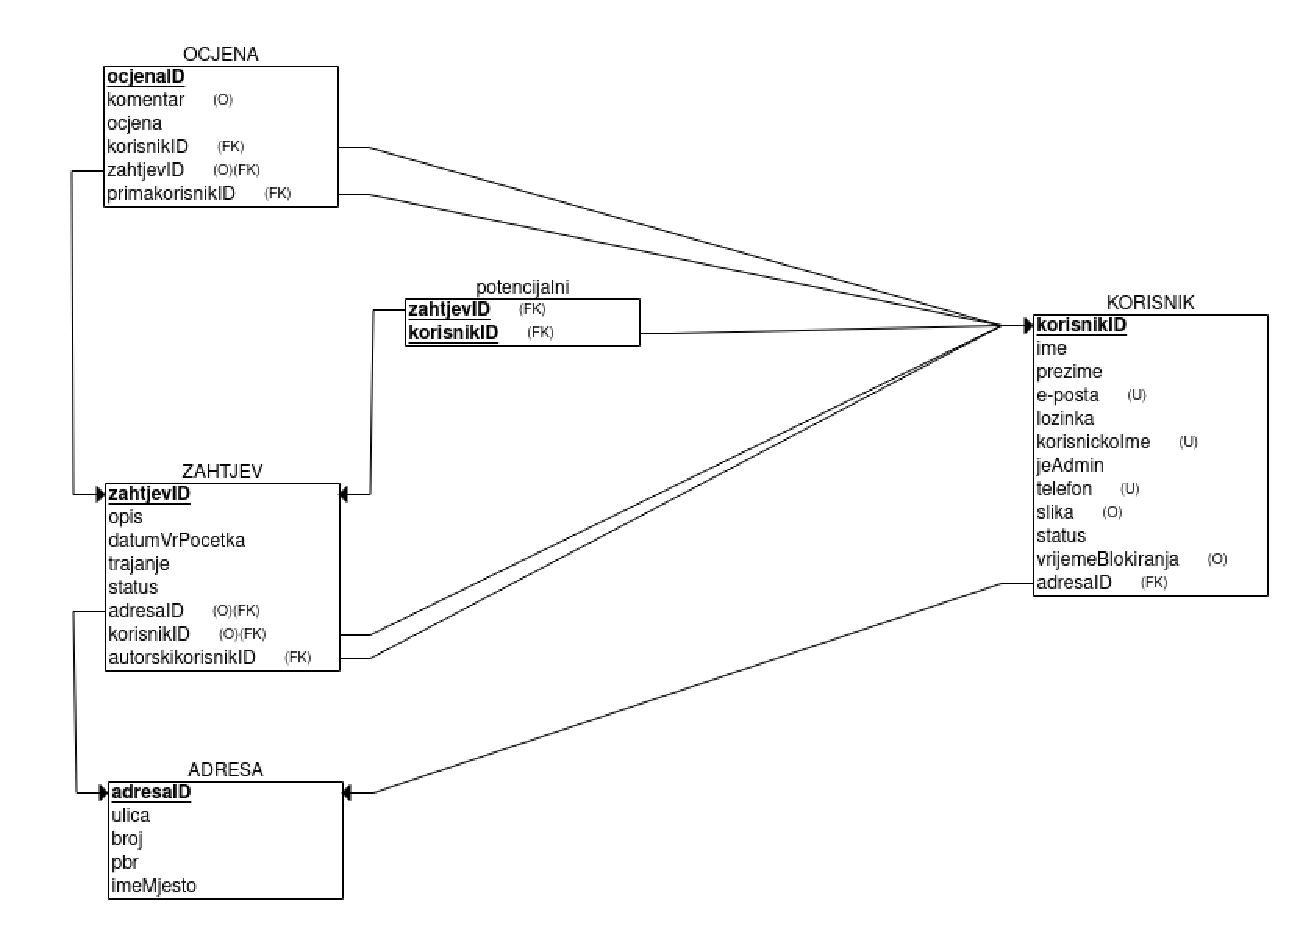
\includegraphics[height=0.45\textheight]{Relacijski_model}
				\caption{Relacijski model baze podataka}
			\end{figure}
			
			\eject
			


			
			
		\section{Dijagram razreda}
		
			U ovom poglavlju opisana je struktura \textit{backenda} aplikacije te opisana glavna funkcionalnost pojedinih klasa.\newline
			\newline
		
		
		
				Na slici 4.3 prikazana je konfiguracija aplikacije \textit{Pomozi mi}. Konfiguracija aplikacije temelji se na postavkama u klasi \textit{WebSecurity}, kojom su definiranja dopuštenja pristupa za pojedini \textit{path}, ponašanje pri \textit{loginu} i \textit{logoutu}. \\
				Klasom RestExceptionHandler regulirano je ponašanje sustava pri pojavi iznimke. Pojava iznimki rezultira \textit{responseom} u kojem je sadržana poruka iznimke.
				
				\begin{figure}[H]
					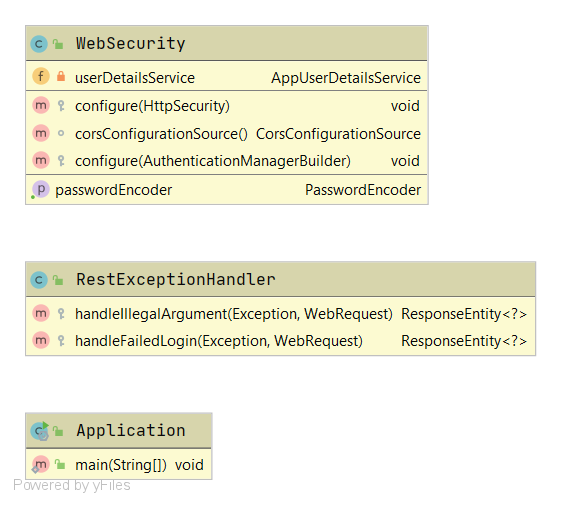
\includegraphics[scale=0.6]{slike/cs1.png} %veličina slike u odnosu na originalnu datoteku i pozicija slike
					\centering
					\caption{Struktura aplikacije i konfiguracija}
					
				\end{figure}
			
				\newpage
				
				Glavni preduvjet za obavljanje bilo kakve aktivnosti unutar aplikacije je da korisnik ima izrađen korisnički račun i prijavljen je u sustav. Klasom \textit{RegistrationDTO} modeliraju se podaci koje korisnik unosi prilikom registracije. Podaci takvog objekta služe kao predložak za stvaranje korisničkog računa. Za prijavu u sustav, provjeru korisničkog imena i lozinke te dodjeljivanje uloga zadužena je klasa \textit{AppUserDetailsService}. Korisniku može biti dodjeljena uloga ROLE\_USER i ROLE\_ADMIN kojima su određene ovlasti 
				slanja zahtjeva na kontrolere.
				
				
				\begin{figure}[H]
					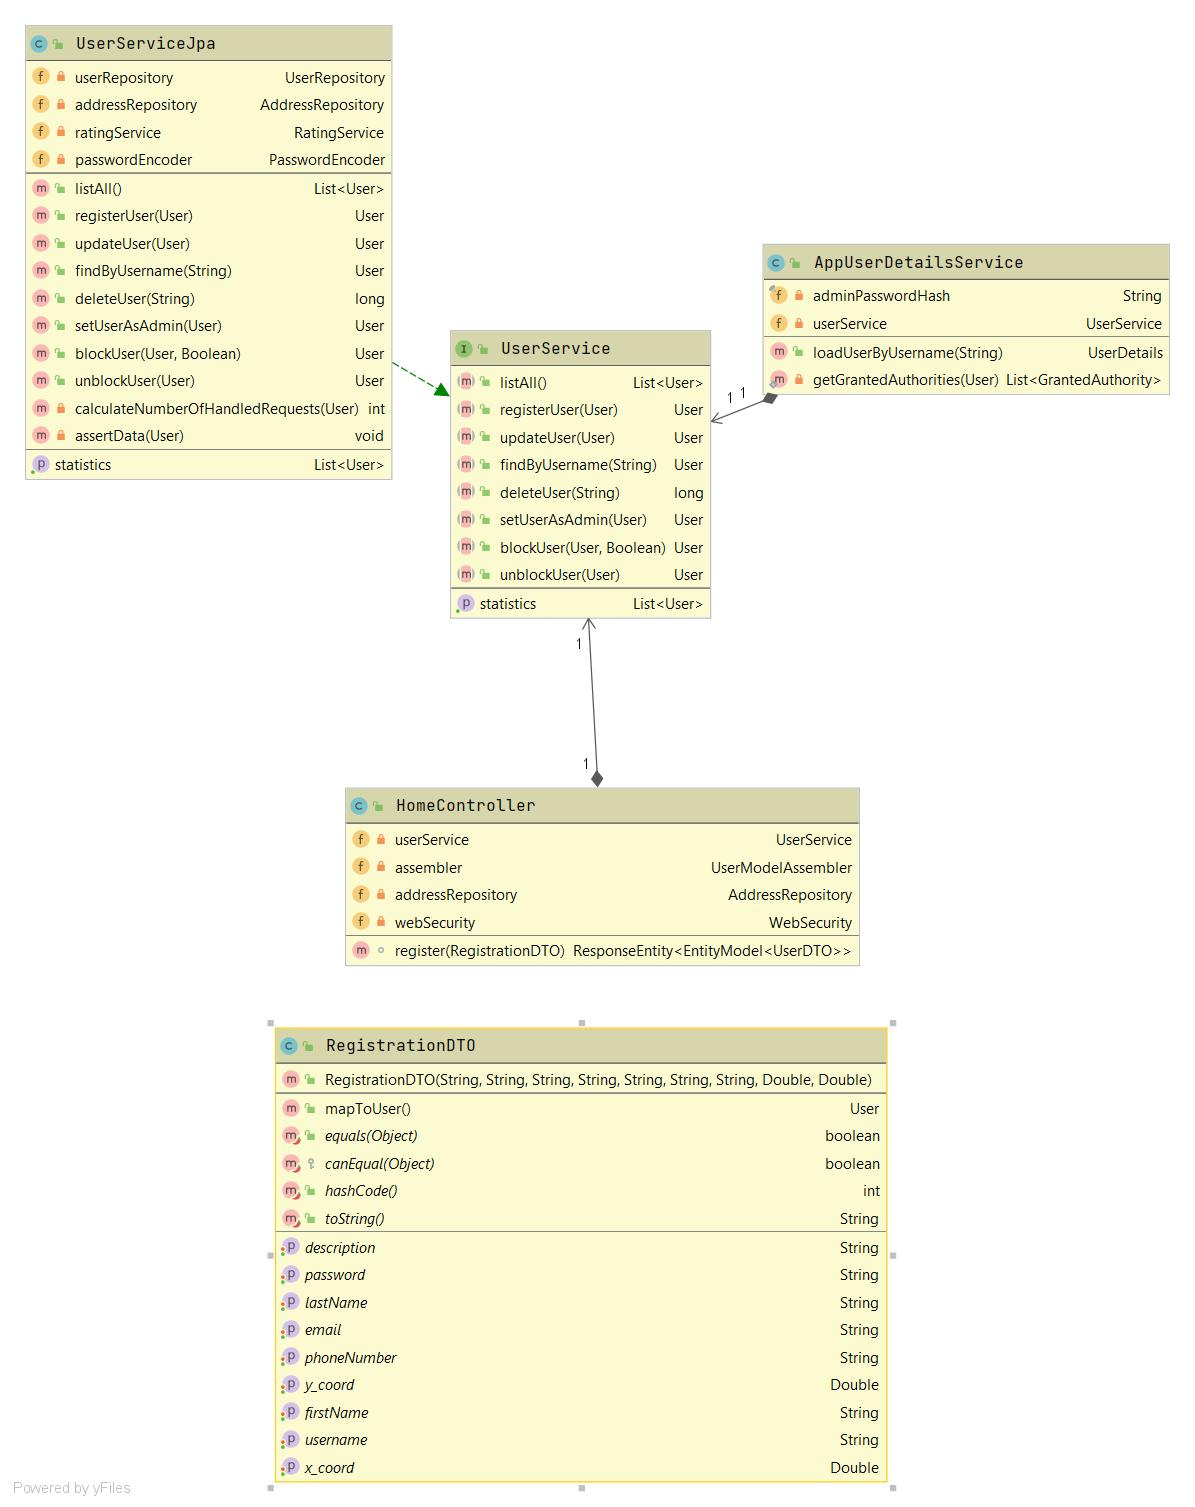
\includegraphics[scale=0.45]{slike/cs4.jpg} %veličina slike u odnosu na originalnu datoteku i pozicija slike
					\centering
					\caption{Klase koje reguliraju registraciju i prijavu}
					
				\end{figure}
			
				\newpage
				
				Slika 4.5 sadržava klase koje su ključne za aktivnosti i rad s korisnicima.
				Klasa \textit{User} predstavlja sam entitet kojim je opisan pojedini korisnik. Sadržava sve relevantne atribute za opis korisnika, konstruktore te funkciju \textit{mapToUserDTO} kojom se objekt \textit{User} pretvara u objekt pogodniji za komunikaciju sa \textit{frontendom}. \textit{UserDTO} predstavlja glavni model komunikacije s vanjskim korisnikom te skriva informacije o pojedinom \textit{Useru} koje nisu relevantne za prikaz na \textit{frontendu}.
				Omogućena je i pretvorba u suprotnom smjeru, iz klase \textit{UserDTO} u klasu \textit{User}. Klasa \textit{UserModelAssembler} omata klasu \textit{UserDTO} u oblik najprikladniji za interaktivnost prikaza, uključujući dodatne linkove. 
				Pristup i manipulacija zapisima korisnika u bazi podataka ostvaren je klasom \textit{UserRepository} koja sadrži sve standardne metode za rad sa zapisima.
				Poslovna logika koja se tiče korisnika ostvarena je u klasi \textit{UserServiceJpa}.
				\textit{UserController} zadužen je za obrađivanje zahtjeva. On inicijalizira komunikaciju sa servisom i bazom podataka i oblikuje podatke o korisnicima u odgovor na zahtjev.
				
				
			
				\begin{figure}[H]
				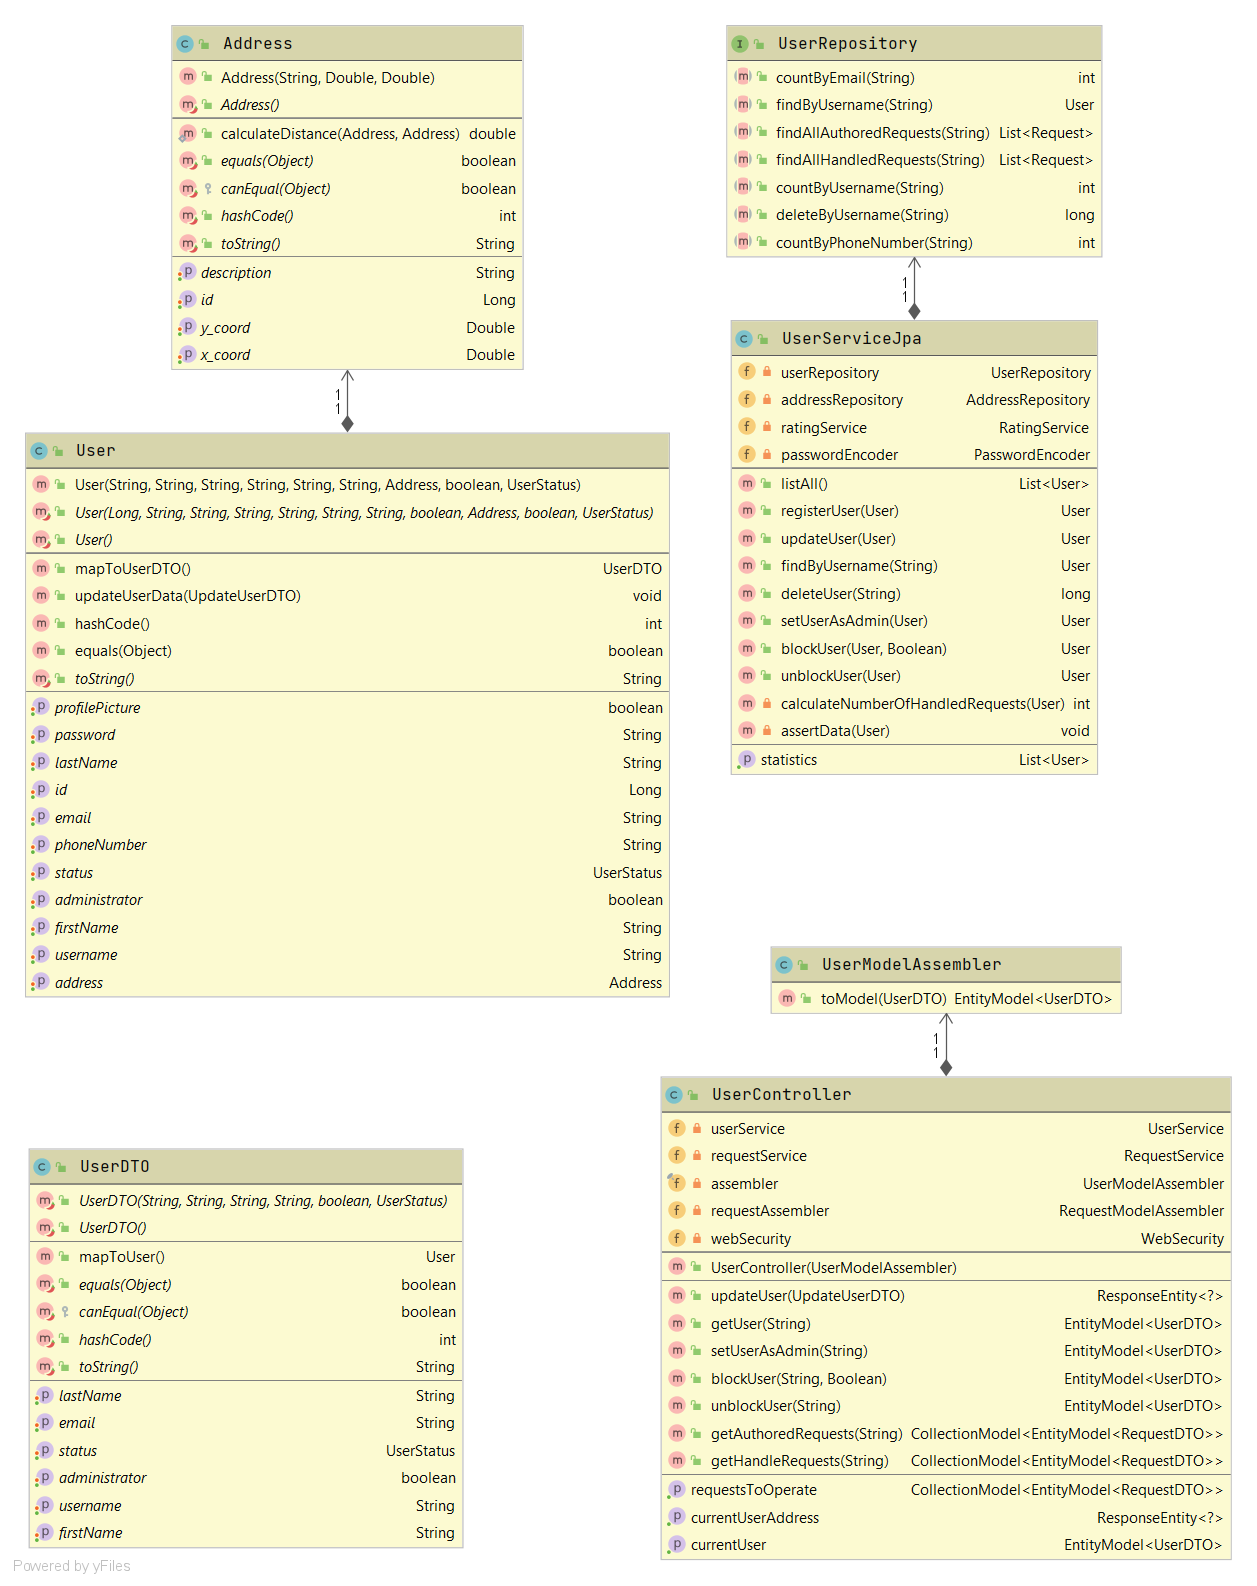
\includegraphics[scale=0.38]{slike/cs2.png} %veličina slike u odnosu na originalnu datoteku i pozicija slike
				\centering
				\caption{Klase koje reguliraju rad s korisnicima sustava}
				
				\end{figure}
			
				\newpage
				
				Klasa \textit{Request} modelira zahtjeve korisnika. Kao i u slučaju sa klasom \textit{User}, ova klasa ima pripadajuću klasu DTO-a, repozitorija, servisa i kontrolera. 
				Prilikom zadavanja zahtjeva, na kontoroler dolazi zahtjev koji u tijelu sadržava objekt tipa \textit{CreateRequestDTO} koji sadrži isključivo podatke koje unosi sam korisnik. Taj objekt je potrebno stvoriti objekt tipa \textit{Request} koristeći dobivene podatke i predefinirane podatke koji opisuju stanje zahtjeva kako bi se on mogao spremiti u bazu podataka.
				
				
			
				\begin{figure}[H]
					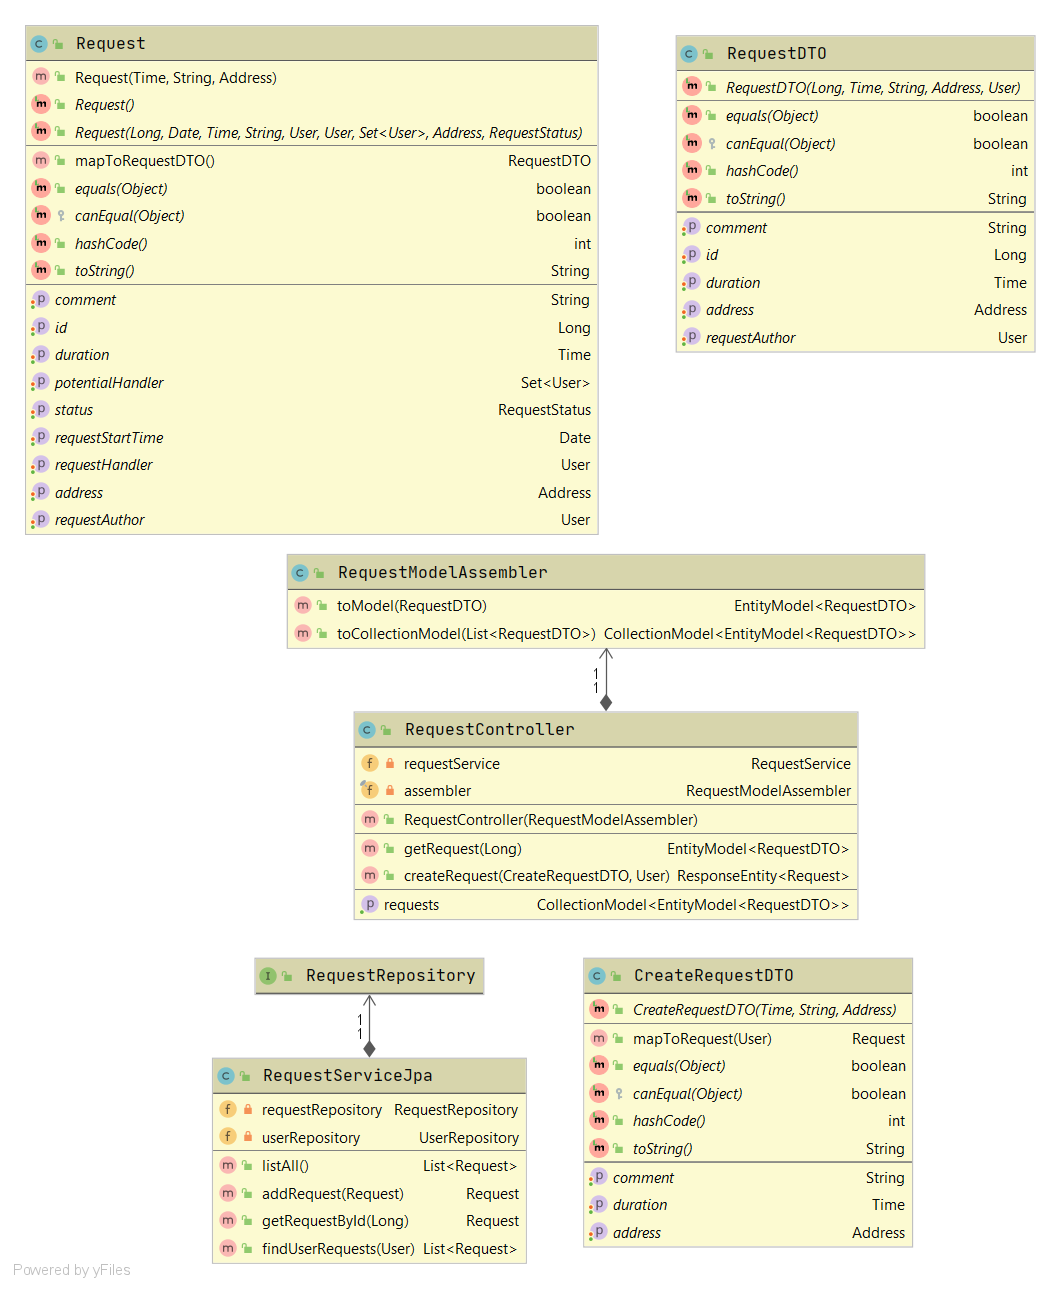
\includegraphics[scale=0.38]{slike/cs3.png} %veličina slike u odnosu na originalnu datoteku i pozicija slike
					\centering
					\caption{Klase koje reguliraju rad sa zahtjevima}
					
				\end{figure}
			
				\newpage
				
				Korisnicima je omogućeno međusobno ocjenjivanje te su na slici 4.7 prikazane klase koje služe modeliranju ocjena i ocjenjivanja. Svaka instancla klase \textit{RatingDTO} ima postavljenog korisnika koji je ocjenjen,ocjenu, komentar te opcionalno zahtjev na koji se odnosi.
				\textit{RatingServiceJpa} omogućuje prikaz ocjena koje je pojedini korisnik autorirao te ocjena koje je pojedini korisnik dobio.			
				\begin{figure}[H]
					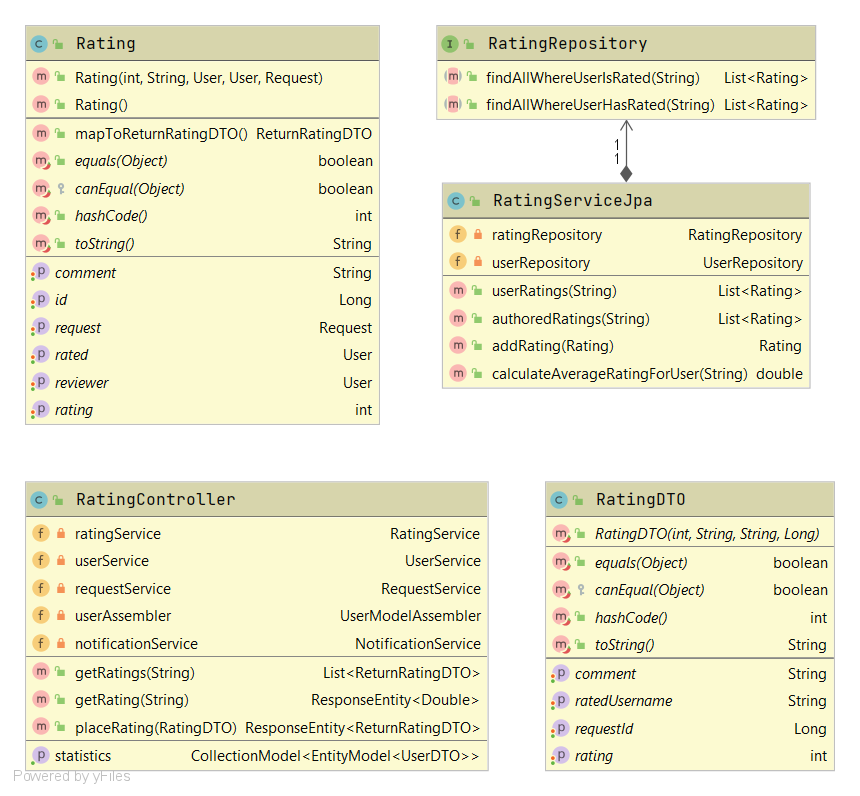
\includegraphics[scale=0.6]{slike/cs5.png} %veličina slike u odnosu na originalnu datoteku i pozicija slike
					\centering
					\caption{Klase koje reguliraju ocjenjivanje korisnika}
					
				\end{figure}
			
				\newpage
			
				Korisnicima za razne aktivnosti sudjelovanja na stranici(stvaranje zahtjeva, javaljanje na zahtjev i mnogi drugi) dolaze obavijesti. Na slici 4.8 prikazane su sve klase koje služe za modeliranje i funkcioniranje obavijesti. Razred \textit{Notification} modelira jednu obavijest. Razred \textit{NotificationDTO} sadrži sve informacije kako bi se obavijest poslala korisniku, tj. sadrži korisnika kojemu je obavijest namijenjena, status obavijesti, poruku koju obavijest nosi, zahtjev za koju je obavijest vezana i na kraju jeli korisnik pročitao obavijest. Kao i razred \textit{Request} sadrži pripadajuće razrede repozitorija, servisa, kontrolera i DTO-a za stvaranje(\textit{CreateNotificationDTO}).
				.			
				\begin{figure}[H]
					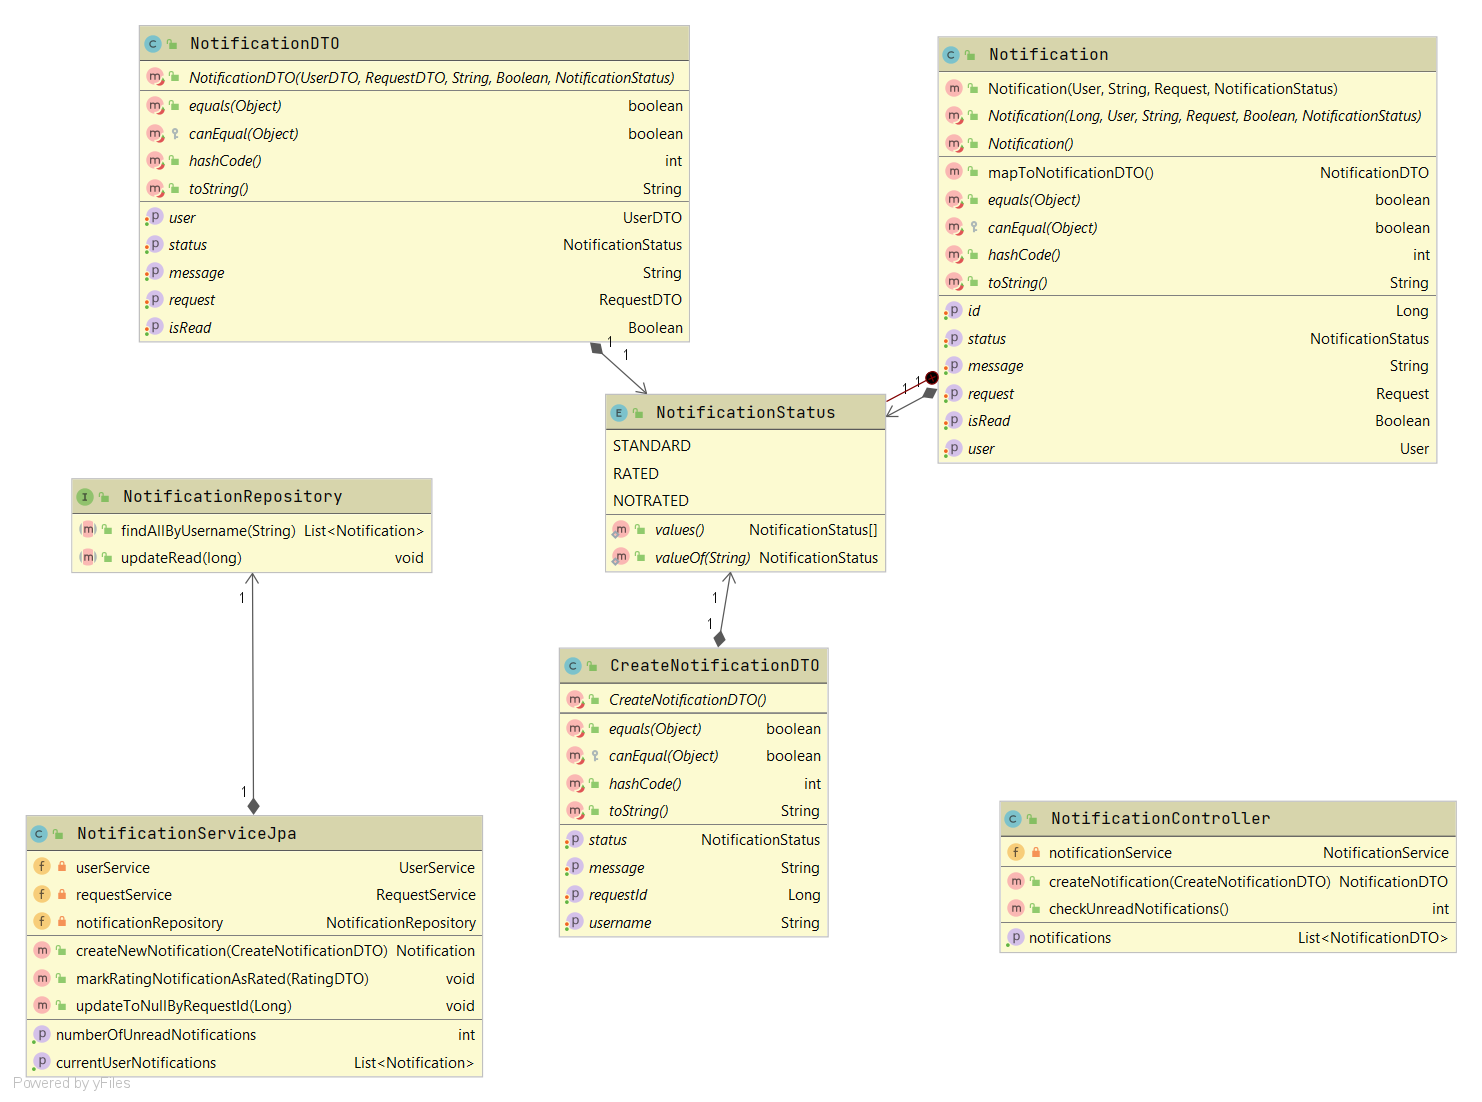
\includegraphics[scale=0.35]{slike/cs6.png} %veličina slike u odnosu na originalnu datoteku i pozicija slike
					\centering
					\caption{Klase koje reguliraju obavijesti}
					
				\end{figure}
				
				
			
				
			
			
				
		
			
			
			\eject
			
		\section{Dijagram stanja}


			Dijagram stanja je tip dijagrama koji služi za opis ponašanja sustava pomoću stanja u koja se može preći nekim događajem. Na slici 4.8 prikazan je dijagram stanja jednog korisnika(koji nije administrator).Nakon prijave(ili registracije ako korisnik nema korisnički račun), korisnik odlazi na početnu stranicu aplikacije. Na početnoj stranici korisnik može: pregledati vlastiti profil, pregledati vlastite zahtjeve, pregledati profile i zahtjeve drugih korisnika, te pregledati statistiku. Klikom na "Pregled profila" korisniku se otvara vlastiti profil, te ga može izbrisati ili izmijeniti. Klikom na "Moji zahtjevi" korisnik može pregledati vlastite zahtjeve. Uz to može stvoriti novi zahtjev, blokirati postojeći, pregledati potencijalne izvršitelje nekog zahtjeva(i time prihvatiti ili odbiti nekog od potencijalnih izvršitelja) i na kraju postaviti zahtjev kao izvršen(i ocijeniti izvršitelja zahtjeva).
			Klikom na "Zahtjevi" korisniku se omogućuje pregled zahtjeva drugih korisnika i samim time se omogućava javljanje za zahtjeve. Klikom na "Profil" korisniku se otvara profil korisnika kojeg želi pregledati, te može vidjeti cjelokupnu ocjenu tog korisnika i sam ga može ocijeniti. Na kraju korisnik može pregledati i statistiku klikom na "Statistika" gdje se prikazuju 3 najbolje ocijenjena korisnika. 
			
			\begin{figure}[h]
				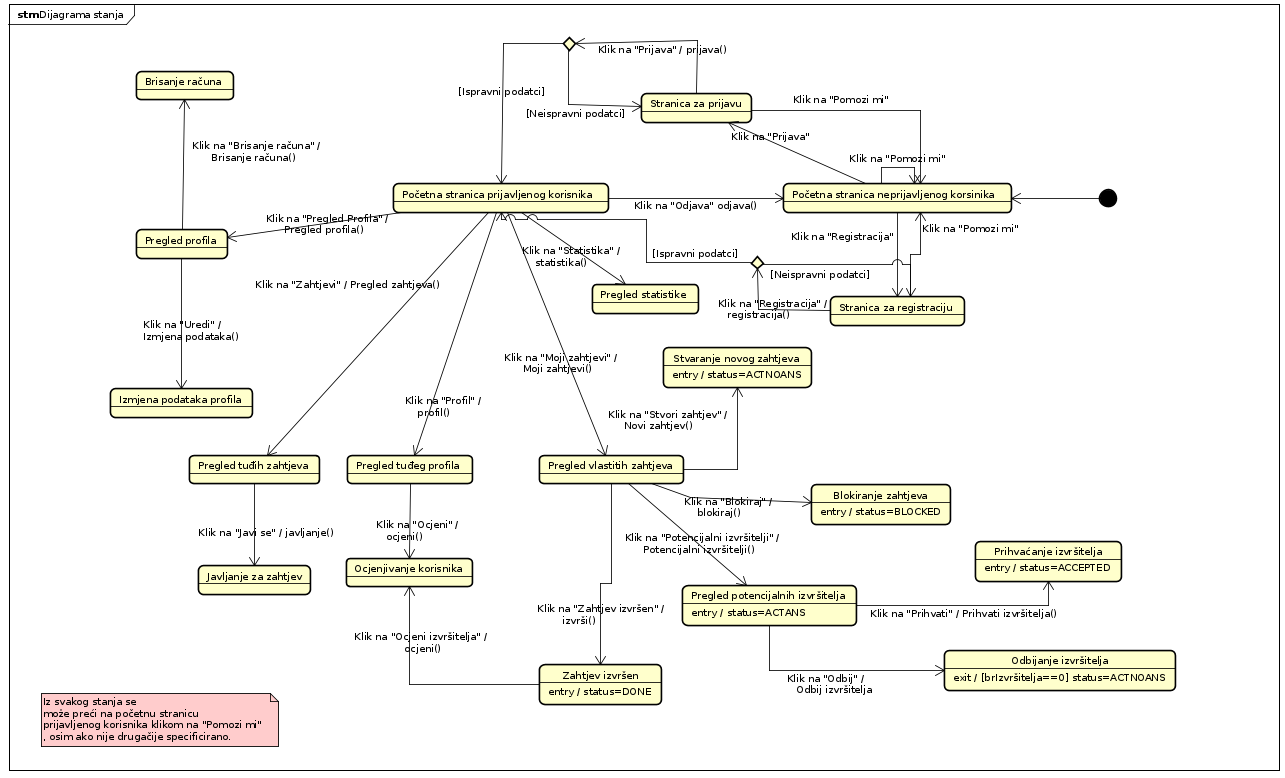
\includegraphics[height=0.47\textheight]{DijagramStanja}
				\caption{Dijagram stanja}
			\end{figure}
			
			\eject 
		
		\section{Dijagram aktivnosti}
		
			Slika 4.8 prikazuje aktivnost korisnika izvršitelja (ubuduće korisnik) pri javljanju na jedan aktivni zahtjev. Na početku aktivnosti korisnik pregledava aktivne zahtjeve i nije autor tih zahtjeva. Nakon toga zadaje radijus koji će se koristiti za prikaz samo onih zahtjeva koji su unutar tog radijusa u odnosu na korisnikovu lokaciju. Ukoliko nema takvih zahtjeva, korisniku se prikaže poruka da nema aktivnih zahtjeva i aktivnost se završava. Ukoliko ima takvih zahtjeva oni se prikazuju korisniku, te se čeka njegov odabir. Ukoliko korisnik ne želi odabrati zahtjev, akcija se tu završava. Ukoliko korisnik odabere neki od tih zahtjeva, korisnik će biti evidentiran kao potencijalni izvršitelj.
		
			
			\begin{figure}[H]
				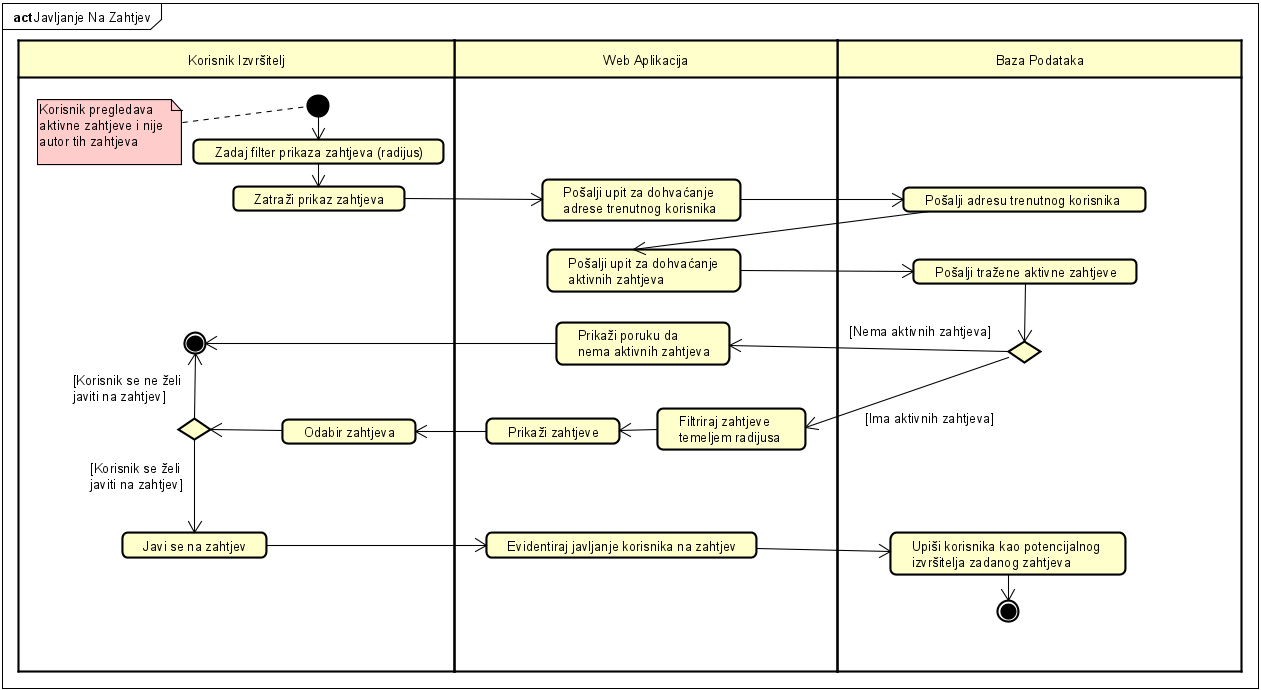
\includegraphics[scale=0.6]{slike/dijagram_aktivnosti.png} %veličina slike u odnosu na originalnu datoteku i pozicija slike
				\centering
				\caption{Aktivnost javljanja na zahtjev}
				
			\end{figure}
			
			\eject
			
		\section{Dijagram komponenti}
		
			Pomoću dijagrama komponenti prikazanog na slici 4.9 prikazan je međuodnos glavnih komponenti sustava.
			Najgrublja podjela komponenata koje međusobno komuniciraju u \textit{ModelViewController} (MVC) obrascu je na:
			\begin{itemize}
				\item Model koji predstavlja skup svih entiteta koji se spremaju u bazi te se nad njima vrše operacije.
				\item View kojeg predstavlja komponenta Frontend web aplikacija.
				\item Controller koji služi za primanje HTTP zahtjeva i slanje odgovora.
			\end{itemize}
			
			Frontend web aplikacija komunicira sa ostatkom aplikacije pri posluživanju statičkog sadržaja poput HTML, CSS i JS datoteka te sa backend dijelom aplikacije u formatu JSON.
			Posluživanje sadržaja frontend dijelu aplikacije ovisi o ulozi korisnika kojemu se poslužuje te
			shodno ulozi komponenta Router odlučuje o tome koje se datoteke poslužuju. Također, u to su uključene i datoteke JavaScript libraryja React koji se koristi u oblikovanju korisničkog sučelja.
			
			Format JSON glavni je format za komunikaciju sa REST API-jem kojeg aplikacija koristi.
			REST API po primitku JSON objekta mapira ga u pripadajući objekt u Javi. Vrijedi i obrnuto, prilikom slanja Java objekta on se prethodno pretvara u pripadajući JSON i u tom obliku šalje HTTP protokolom.
			
			
			Komponenta kontrolera putem DTO objekata ostvaruje komunikaciju sa REST API-jem i poslovnom logikom aplikacije.
			Pristup bazi na backendu nudi se sučeljem s komponentom \textit{JPARepositories} 
			te ona služi kao glavna komunikacija aplikacije i SQL baze podataka u jeziku JPQL.
			
			 \begin{figure}[H]
			 	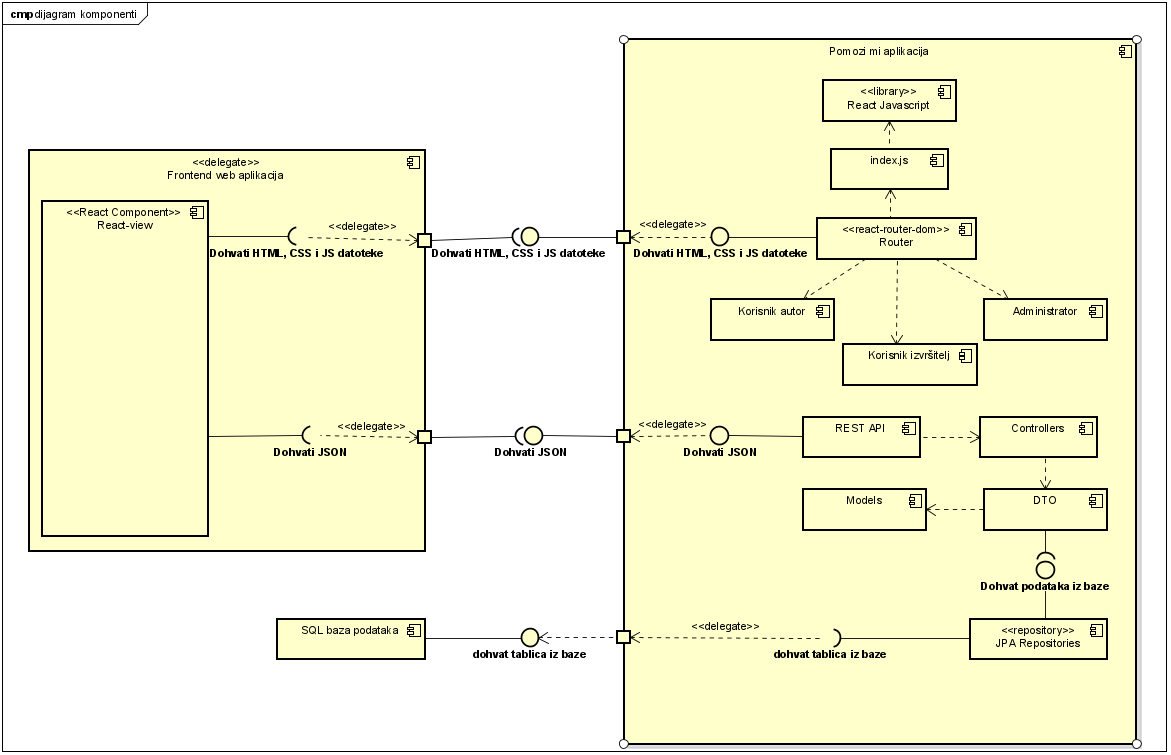
\includegraphics[height=0.5\textheight]{dijagramKomponenti}
			 	\caption{Dijagram komponenti}
			 \end{figure} 
			